\documentclass[a4paper,12px]{article}
\usepackage{graphicx}
\usepackage[english]{babel}
\usepackage{fancyhdr}
\usepackage{lastpage}
\usepackage{xifthen}
\usepackage[linesnumberedhidden, titlenotnumbered]{algorithm2e}
\usepackage{lipsum}
\usepackage{hyperref}
\usepackage{array}
\usepackage{tabularx}
\usepackage{caption}
\usepackage{amsfonts}
\usepackage{amsmath}

\usepackage{minted}
\usepackage{listings}
\renewcommand\listingscaption{}

\pagestyle{fancy}
\lhead{
\includegraphics[width=7cm]{logoUvA}}
\rhead{\footnotesize \textsc {Report\\ \opdracht}}
\lfoot
{%
    \footnotesize \studentA
    \ifthenelse{\isundefined{\studentB}}{}{\\ \studentB}
    \ifthenelse{\isundefined{\studentC}}{}{\\ \studentC}
    \ifthenelse{\isundefined{\studentD}}{}{\\ \studentD}
    \ifthenelse{\isundefined{\studentE}}{}{\\ \studentE}
}
\cfoot{}
\rfoot{\small \textsc {Page \thepage\ of \pageref{LastPage}}}
\renewcommand{\footrulewidth}{0.5pt}

\fancypagestyle{firststyle}
{%
    \fancyhf{}
    \renewcommand{\headrulewidth}{0pt}
    \chead{
\includegraphics[width=7cm]{logoUvA}}
    \rfoot{\small \textsc {Page \thepage\ of \pageref{LastPage}}}
}

\setlength{\topmargin}{-0.3in}
\setlength{\textheight}{630pt}
\setlength{\headsep}{40pt}

% =================================== DOC INFO ===================================

\newcommand{\titel}{Algorithms and Complexity}
\newcommand{\opdracht}{Week 2: Assignments}
\newcommand{\docent}{Dr. Leen Torenvliet}
\newcommand{\cursus}{Algorithms and Complexity}
\newcommand{\vakcode}{5062ALCO6Y}
\newcommand{\datum}{\today}
\newcommand{\studentA}{Robin Klusman}
\newcommand{\uvanetidA}{10675671}
\newcommand{\studentB}{Maico Timmerman}
\newcommand{\uvanetidB}{10542590}
\newcommand{\studentC}{Boudewijn Braams}
\newcommand{\uvanetidC}{10401040}
\newcommand{\studentD}{Govert Verkes}
\newcommand{\uvanetidD}{10211748}
%\newcommand{\studentE}{Naam student 5}
\newcommand{\uvanetidE}{UvAnetID student 5}

% ===================================  ===================================

\begin{document}
\thispagestyle{firststyle}
\begin{center}
    \textsc{\Large \opdracht}\\[0.2cm]
    \rule{\linewidth}{0.5pt} \\[0.4cm]
    {\huge \bfseries \titel}
    \rule{\linewidth}{0.5pt} \\[0.2cm]
    {\large \datum  \\[0.4cm]}

    \begin{minipage}{0.4\textwidth}
        \begin{flushleft}
            \emph{Supervisor:} \\
            \docent \\[0.2cm]
            \emph{Student:}\\
            {\studentA \\ {\small \uvanetidA \\[0.2cm]}}
            \ifthenelse{\isundefined{\studentB}}{}{\studentB \\ {\small \uvanetidB \\[0.2cm]}}
        \end{flushleft}
    \end{minipage}
    ~%
    \begin{minipage}{0.4\textwidth}
        \begin{flushright}
            \emph{Course:} \\
            \cursus \\[0.2cm]
            \emph{Student:}\\
            \ifthenelse{\isundefined{\studentC}}{}{\studentC \\ {\small \uvanetidC \\[0.2cm]}}
            \ifthenelse{\isundefined{\studentD}}{}{\studentD \\ {\small \uvanetidD \\[0.2cm]}}
            \ifthenelse{\isundefined{\studentE}}{}{\studentE \\ {\small \uvanetidE \\ [0.2cm]}}
        \end{flushright}
    \end{minipage}\\[1 cm]
\end{center}


% =================================== CONTENTS ===================================

\tableofcontents
\clearpage

% =================================== MAIN TEXT ===================================

\section{Assignment 1}
\subsection{Complexity analysis}

% \begin{listing}
%     \inputminted[lastline=45]{python}{1.py}
% \caption{Converting the adjacency matrix to vertex dictionary}
% \end{listing}
% \begin{listing}
%     \inputminted[firstline=46]{python}{1.py}
% \caption{Converting the adjacency matrix to vertex dictionary}
% \end{listing}
% \begin{listing}[H]
% \inputminted{python}{1b.py}
% \caption{}
% \end{listing}

See the code in '1.py' for full implementation (graphs are implemented using the
NetworkX\footnote{\url{https://networkx.github.io/}} python library)


\subsubsection{Naive algorithm}

A naive way to find the shortest path between two vertices in a weighted graph
is by generating a list of all the paths between the two vertices and iterating
over them to determine which is the shortest. Our implementation uses a NetworkX
function to return the list of all non-cyclic paths between two nodes
('all\_simple\_paths') and two additional functions to determine the shortest of
these.

$$V = \text{Set of all vertices in graph}$$
$$E = \text{Set of all edges in graph}$$

According to the NetworkX
documentation\footnote{\url{http://networkx.github.io/documentation/development/reference/generated/networkx.algorithms.simple\_paths.all\_simple\_paths.html}}
their algorithm uses a modified depth-first search the find all possible paths.
Finding a single path using this algorithm is in $O(|V|+|E|)$, this means
finding all paths is in $O(|V|! * (|V|+|E|))$.


Two additional (non NetworkX) functions are used to determine the shortest path
in this list. $calculate\_path\_length$: returns the sum of all edges between two
vertices $O(|V|)$. And $shortest\_path\_in\_list$: returns the shortest path in a
list of paths (using the function above) $O(|V|! * |V|)$


Combining the complexities of these functions combined gives
$O(|V|! * (|V|+|E|) + |V|! * |V|)$, which means the time
complexity of the naive algorithm implemented as described above
is $O(|V|! * (|V|+|E|))$.


\subsubsection{Dijkstra's algorithm}

Put simply, Dijkstra's algorithm attempts to find the shortest path between two
vertices by iterating over subsequent connected vertices ($V_{i}$) starting at the
source. This while keeping track of all path lengths (calculated by adding the
weight of the new edge connecting the previous vertex with $V_{i}$). The time
complexity is therefore $O(|V|^{2})$.

Dijkstra's original implementation makes use of sets (an unordered data
structure by definition). The NetworkX implementation uses a binary heap to
store the vertex
sets\footnote{\url{https://networkx.github.io/documentation/latest/\_modules/networkx/algorithms/shortest\_paths/weighted.html\#single\_source\_dijkstra}}.
Taking advantage of the properties of this data structure the complexity is
reduced to $O(|E| *
log(|V|))$\footnote{\url{http://www.cosc.canterbury.ac.nz/research/reports/HonsReps/1999/hons\_9907.pdf}}.

\newpage

\subsection{Test results}

Finding the shortest path between vertex 0 and 14 in a bidirectional weighted graph, see adjacency matrix below
\begin{listing}[H]
    \inputminted[fontsize=\footnotesize]{text}{inputgraph}
    \caption{Adjacency matrix of the input graph}
\end{listing}

Two sets of three runs were time using the Linux `time' utility, the first set
attempts to find the shortest path using the naive approach, the second uses
Dijkstra's algorithm (as implemented by the NetworkX module).

\begin{listing}[H]
$\text{Naive algorithm} - O(|V|! * (|V|+|E|))$:

\begin{table}[H]
    \begin{tabular}{lll}
        Run 1: &       &          \\
               & real: & 26.814s  \\
               & user: & 26.682s  \\
               & sys:  & 0.153s   \\
        Run 2: &       &          \\
               & real: & 26.562s  \\
               & user: & 26.430s  \\
               & sys:  & 0.153s   \\
        Run 3: &       &          \\
               & real: & 26.371s  \\
               & user: & 26.238s  \\
               & sys:  & 0.151s   \\\\

        \multicolumn{3}{l}{\text{Average (real):} 26.582s}
    \end{tabular}
\end{table}
\end{listing}

\begin{listing}[H]
$\text{Dijkstra's algorithm} - O(|E| * log(|V|))$:

\begin{table}[H]
    \begin{tabular}{lll}
        Run 1: &       &          \\
               & real: & 0.093s   \\
               & user: & 0.077s   \\
               & sys:  & 0.015s   \\
        Run 2: &       &          \\
               & real: & 0.092s   \\
               & user: & 0.077s   \\
               & sys:  & 0.015s   \\
        Run 3: &       &          \\
               & real: & 0.092s   \\
               & user: & 0.077s   \\
               & sys:  & 0.015s   \\\\
        \multicolumn{3}{l}{\text{Average (real):} 0.092s}
    \end{tabular}
\end{table}
\end{listing}

The performance increase when using Dijkstra's algorithm in comparison to the
naive implementation is substantial, which is to be expected when regarding
their respective time complexities.

\section{Assignment 2} $G = (V, E)$ is a graph with $V$ vertices and $E$ edges.
An algorithm for removing the most vital edge, $e$, from the shortest path, $p$
can be written as: $(\forall e \in p)(E' = E - e)(\forall E' $ calculate
Dijkstra over $G' = (V, E'))$. Then the longest shortest path, matches with the
$e$ removed from $p$, where $e$ is the most vital edge in $p$.  The complexity
of this algorithm depends on the length of the shortest path and on Dijkstra's
algorithm: $O(n \cdot |E| + \log_{|V|}{|V|})$.

Using the following code (graphs are implemented using the
NetworkX\footnote{\url{https://networkx.github.io/}} package), we determined that the most vital edge, $e$ in graph
$G$ is edge (0, 11). Making the new shortest path $[0,6,10,7,4,14]$ with a
length of 17 and thereby increasing the length of the shortest path by 2.

\begin{listing}[H]
\inputminted[firstline=4,lastline=32,fontsize=\footnotesize]{python}{2.py}
\caption{Determine the most vital edge}
\end{listing}


\section{Assignment 3}
\subsection{Complexity analysis}
For a undirected graph $G = (V,E)$ with $V$ vertices and $E$ edges, we can define a greedy
algorithm to create a minimum spanning tree. A greedy algorithm is an algorithm that
makes the locally optimal choice at each stage in the algorithm. Using Depth
First Search, we start searching for a cycle in the graph. We then remove this
edge which has the highest weight. By removing this edge we do not take in
account what effect this might have in the rest of the graph. There could have
been an edge which had less weight, but was part of multiple cycle at the same
time.

Depth First Search has a worst case complexity of $O(|E|)$ therefor creating a
minimum spanning tree using the described algorithm has the same complexity,
$O(n)$.

\subsection{Minimum spanning tree}

The Wikipedia entry for `minimum spanning
tree'\footnote{\url{http://en.wikipedia.org/wiki/Minimum\_spanning\_tree}}
implies the term is only applicable to undirected graphs. For this reason the
input graph from exercise 1 is first converted to an undirected graph by only
retaining edges that connect vertices in both directions (arbitrarily selecting
one of the two edge weights). The resulting minimum spanning tree has a total
weight of 289.

\begin{listing}[H]
    \inputminted[fontsize=\footnotesize]{text}{inputgraph}
    \caption{Adjacency matrix of the given graph}
\end{listing}

\begin{listing}[H]
    \inputminted[fontsize=\footnotesize]{text}{inputgraph2}
    \caption{Adjacency matrix of the input graph converted to an undirected graph}
\end{listing}

\begin{listing}[H]
    \inputminted[fontsize=\footnotesize]{text}{inputgraph3}
    \caption{Minimum spanning tree of the input graph}
\end{listing}

\begin{figure}[H]
    \centering
    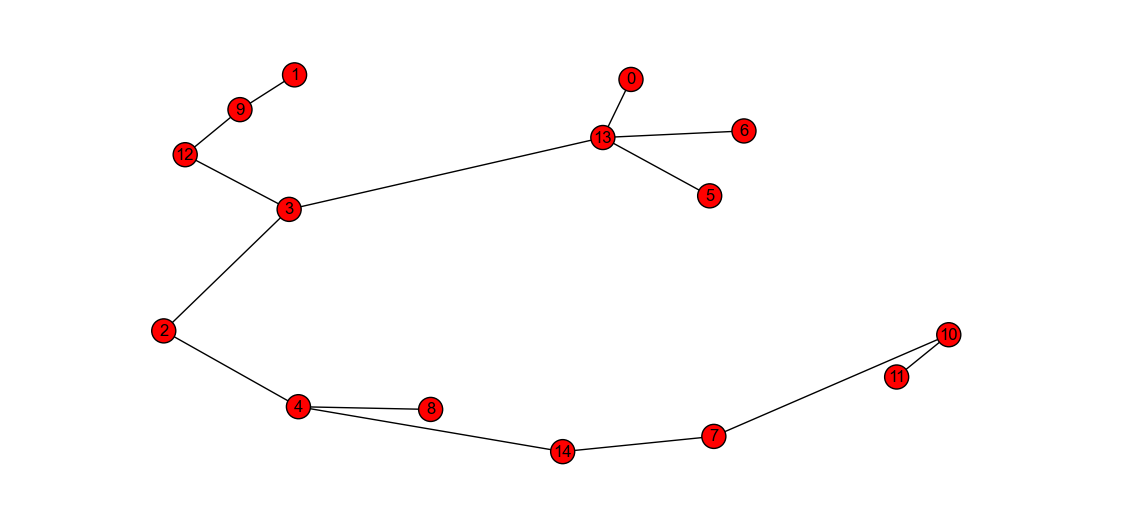
\includegraphics[width=\textwidth]{figure_1.png}
    \caption{Visual representation of the minimum spanning tree}
\end{figure}

\section{Assignment 4}

One possible approach to solving this problem is to brute force through all the
possible independent sets with a divide and conquer algorithm until you've found
one larger than the specified k.

\begin{enumerate}
    \item{Repeat all the following steps for every vertex $i$ in the graph $G$.}
    \item{For a vertex $j$, remove all its neighbours from the graph.}
    \item{Add vertex $j$ to the independent set.}
    \item{If $j$ was the only vertex in in the graph after eliminating all neighbours.
            The algorithm is finished.}
    \item{If there are more vertices in the graph after eliminating all
        neightbours of $j$, apply the same algorithm recursively, with the graph $G' =
    G - \{ i, \text{neighbours(i)} \}$ }
\end{enumerate}

The algorithm needs to be applied to all vertexes, giving it the complexity of
$O(|V| * f(n))$, where f(n) is finding the maximum independent set of a graph
with starting vertex $v$.

$$T(n) =
    \left\{
        \begin{array}{ll}
            1 & n < 2  \\
            (n - 1 - k) * T(n-k) + c &  n \geq 2 \\
        \end{array}
    \right.$$

f(n) has the complexity of $O(|V| \cdot 2^{|V|})$ because of the following
recurrence relation. Here n is equal to |V| and k is equal to the neighbours of
vertex $v$. This results in our algorithm having a complexity of $O(|V|^{2}
\cdot 2^{|V|})$

Because this algorithm has exponential complexity, calculating for big graphs
can not be done within finite time.

% The complexity of this algorithm would be O(n^2 * n!).
% Factorial since all the different permutations of the grandchildren have to be checked each time.
%
% The reason I believe there is no question about the graph of assignment 1 is because this problem is a NP-hard problem and thus rather difficult to implement in an efficient way.
% \begin{listing}
% \inputminted{python}{4.py}
% \caption{Maximum sum path}
% \end{listing}

% =================================== REFERENCES ===================================

%\clearpage
%\bibliographystyle{unsrt}
%\bibliography{bib}

\end{document}
